\begin{frame}
\frametitle{Document Examiner}
\begin{itemize}
	\item 1985
	\item Symbolics Inc.
	\item Symbolics Handbücher
	\item Concordia als Editor
\end{itemize}

\begin{figure}[htbp]
	\centering
	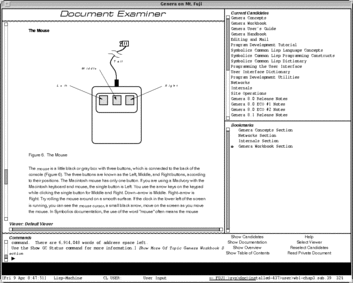
\includegraphics[width=0.5\textwidth]{images/documentExaminer}
\end{figure}

\end{frame}

\begin{frame}
\frametitle{Document Examiner}
\framesubtitle{Funktionen}
	\begin{itemize}
		\item Userinterface / Bedienmöglichkeiten
		\begin{itemize}
			\item An die Recherche in Handbüchern angepasst
			\item Content area, Kandidaten, Bookmarks, Command region
			\item Ein Klick auf einen Link fügt zu Kandidaten hinzu
		\end{itemize}
		\item Links / Strukturen
		\begin{itemize}
			\item Inspiriert von NLS, Xanadu und HES
			\item Records enthalten Titel und Beschreibung
			\item Record hat ID
			\item Sequenzen von Records
		\end{itemize}
	\end{itemize}
\end{frame}